\documentclass[10pt,twocolumn]{article}
\usepackage{graphicx}
\usepackage[margin=0.5in]{geometry}
\usepackage[cmex10]{amsmath}
\usepackage{array}
\usepackage{booktabs}
\usepackage{mathtools}
\title{\textbf{Optimization Advanced}}
\author{Vemulapalli Bavya Sri}
\date{October 2022}
\providecommand{\norm}[1]{\lVert#1\rVert}
\providecommand{\abs}[1]{\vert#1\vert}
\let\vec\mathbf
\newcommand{\myvec}[1]{\ensuremath{\begin{pmatrix}#1\end{pmatrix}}}
\newcommand{\mydet}[1]{\ensuremath{\begin{vmatrix}#1\end{vmatrix}}}
\providecommand{\brak}[1]{\ensuremath{\left(#1\right)}}
\providecommand{\lbrak}[1]{\ensuremath{\left(#1\right.}}
\providecommand{\rbrak}[1]{\ensuremath{\left.#1\right)}}
\providecommand{\sbrak}[1]{\ensuremath{{}\left[#1\right]}}



\begin{document}
\maketitle
\paragraph{\textit{Problem Statement} - If $\frac{dy}{dx} = x(x-1)^2(x-3)^3$, show that $x=0$ gives a maximum value to $y$ and $x=3$ gives a minimum.}

\section{Solution}
\begin{flushleft}
Given function is,\\
\begin{equation}
    \nabla f(x) = x(x-1)^2(x-3)^3
\end{equation}
\end{flushleft}


\subsection{Calculation of Maxima using gradient ascent algorithm}

To find:
\begin{align}
\max_{x} f(x)
\end{align}  
\begin{flushleft}
Maxima of the above equation (1), can be calculated from the following expression,
\end{flushleft}

    \begin{equation}
        x_{n+1}= x_n + \alpha \nabla f(x_n)
    \end{equation}
\begin{flushleft}
Taking $x_0=0,\alpha=0.001$ and precision = 0.00000001, values obtained using python are:
\end{flushleft} 
\center
        \boxed{$\text{Maxima} = 0$}\\
        \vspace{0.45cm}
        \boxed{$\text{Maxima Point} = 1$}
\endcenter
\begin{flushleft}
\subsection{Calculation of Minima using gradient descent algorithm}
\end{flushleft}
\begin{flushleft}
To find:
\end{flushleft}
\begin{align}
\min_{x} f(x)
\end{align}  
\begin{flushleft}
Minima of the above equation (1), can be calculated from the following expression,\\
\end{flushleft}
    \begin{equation}
        x_{n+1}= x_n - \alpha \nabla f(x_n) 
    \end{equation}
\begin{flushleft}
Taking $x_0=3,\alpha=0.001$ and precision = 0.00000001, values obtained using python are:
\end{flushleft}
\center
        \boxed{$\text{Minima} = 0$}\\
        \vspace{0.45cm}
        \boxed{$\text{Minima Point} = 3$}
\endcenter
\section{Plot to find maxima and minima of the function}
\vspace{0.25cm}
Plot of the function $\frac{(x^2-7x+6)}{(x-10)}$ is shown in the figure 1.
\begin{figure}[h]
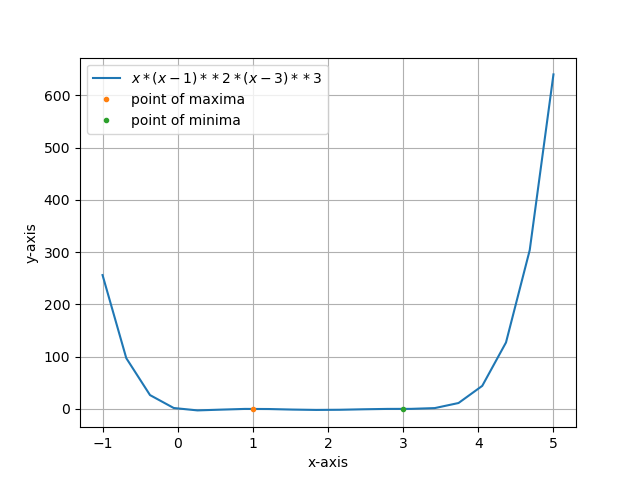
\includegraphics[width=1\columnwidth]{opt.png}
\caption{Plot of df(x) to find Maxima and Minima}
\label{Optimization of Machince A and B}
\end{figure}

\section{Conclusion}
\begin{flushleft}
Maxima and Minima and related points are, \\
\vspace{0.25cm}
\center
\boxed{$\text{Maxima point, Max} = (1 , -2)$} \\
\vspace{0.25cm}
and \\
\vspace{0.25cm}
\boxed{$\text{Minima point, Min} = (3 , -2)$}
\endcenter
\end{flushleft}
\end{document}